\chapter{Experiments} \label{Experiments}
 
\section{Experiment 1}
The first experiment was conducted on a fully synthetic dataset. Supervised and unsupervised learning approaches were used to detect the anomalies. 

\subsection{Dataset} \label{dataset1}
The dataset, that was created for this first task consisted of five variables. The dataset was created under the assumption, that one measurement was drawn per hour on totally 2000 days, resulting in 48000 datapoints. The variables all follow a cyclic pattern shown in Figure \ref{fig:synthetic data} but are not dependent on each other. 

\begin{figure}[h]
	\centering
	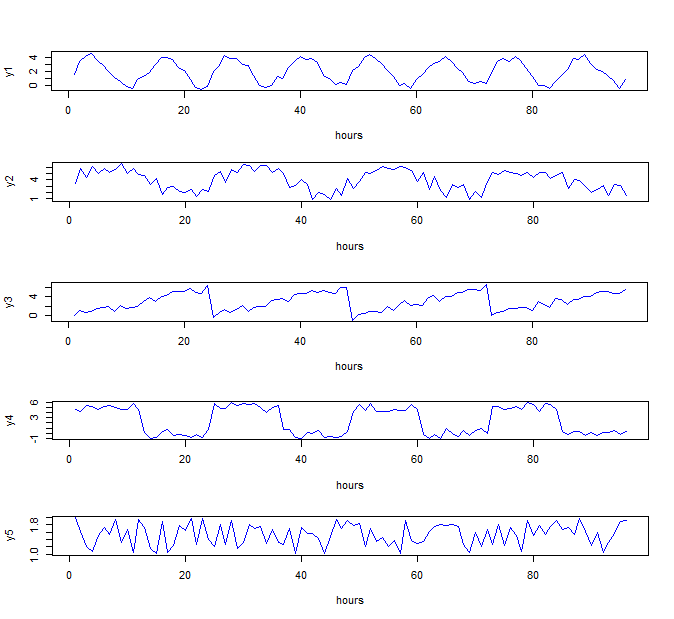
\includegraphics[scale=0.7]{Figures/synthetic data}
	\decoRule
	\caption[Synthetic Dataset]{Synthetic Dataset \parencite{own}}
	\label{fig:synthetic data}
\end{figure}

In a second step the dataset was enriched with six different kinds of anomalies. The anomalies embedded into the dataset are of type deviant cycle, temporary change and level shift. Figure \ref{fig:anomalies} shows examples of the embedded anomalies. The same kind of anomalies were embedded into the training and the test dataset.

\begin{figure}[h]
	\centering
	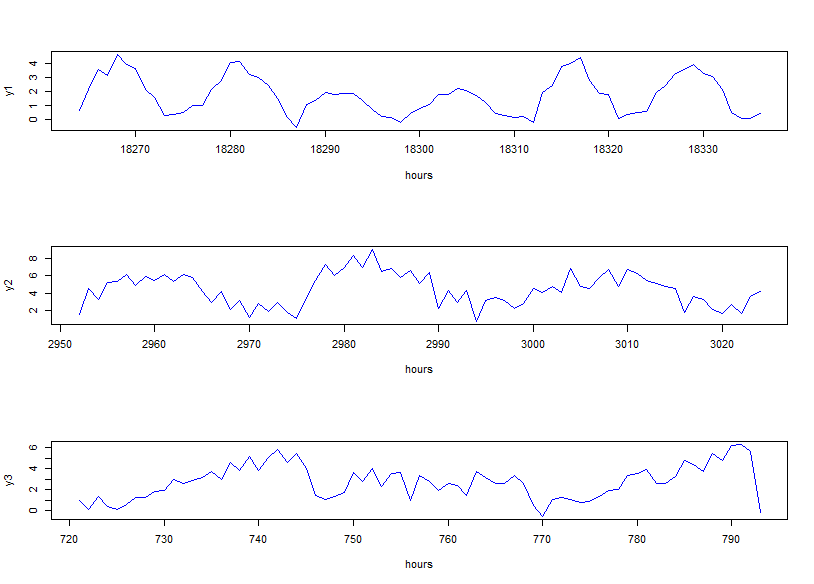
\includegraphics[scale=0.7]{Figures/Anomalies}
	\decoRule
	\caption[Synthetic Anomalies]{Synthetic Anomalies \parencite{own}}
	\label{fig:anomalies}
\end{figure}

For the supervised learning approach the dataset was also labelled. In each case the whole day was marked as an anomaly. In total 30 anomalous days were embedded into the dataset, this corresponds to 1.5 percent of anomalous datapoints.

\subsection{Neural Networks}
In the first experiment, a CNN was tested against a RNN in a supervised and also in an unsupervised fashion. As RNN, the type GRU was chosen. As some first attempts showed, that it showed sufficient results with improved computation time compared to the more complex LSTM. 

For the supervised learning approach, the chosen architecture can be seen in table \ref{Tab:Supervised Learning1}. The architecture with two hidden layers, first presented in Section \ref{Anomaly Detection on Univariate Time Series}, served as example for the RNN. Supplementary, the CNN was built to match the number of layers used for the RNN, where each convolutional layer was followed by a max-pooling layer (explained in Section \ref{CNN}.     

\begin{table}[h]
\caption{Configuration of Supervised Learning in Exp. 1 }
	\begin{center}
		\begin{tabular}{ | c | c | c | c |}
			\hline
			\thead{} & \thead{Input} & \thead{NN-Architecture} & \thead{Output} \\
			\hline
			\thead{CNN} &  120 past datapoints  & \makecell{2 1D-Convolutional Layers \\ 2 Max-Pooling Layers \\ 1 Dense Layer}  & \makecell{1 Dense Layer \\ with Sigmoid Activation}   \\
			\hline
			\thead{RNN} &  120 past datapoints  & \makecell{2 GRU Layers \\ 1 Dense Layer}  & \makecell{1 Dense Layer \\ with Sigmoid Activation}  \\
			\hline
		\end{tabular}
		\label{Tab:Supervised Learning1}
	\end{center}
\end{table}

 
The architecture used for the unsupervised learning approach, displayed in table \ref{Tab:Unupervised Learning1}, looked very similar to the architecture of the supervised approach. The main difference between the two architectures was that the CNN was not built as a sequential model, because the used software does not support such an architecture. Instead of having one output layer, the CNN had to be designed with five parallel output layers, each predicting one time series \footnote{More detailed summaries of the models can be found in appendix \ref{AppendixA}}. In comparison, the RNN has just one output layer with 5 neurons, each used to predict a time series.    

\begin{table}[h]
	\caption{Configuration of Unupervised Learning in Exp. 1}
	\begin{center}
		\begin{tabular}{ | c | c | c | c |}
			\hline
			\thead{} & \thead{Input} & \thead{NN-Architecture} & \thead{Output} \\
			\hline
			\thead{CNN} &  120 past datapoints  & \makecell{2 1D-Convolutional Layers \\ 2 Max-Pooling Layers }  & \makecell{ 5 Dense Layers with \\ 1 regression outputs}   \\
			\hline
			\thead{RNN} &  120 past datapoints  & \makecell{2 GRU Layers}  & \makecell{ 1 Dense Layers with \\ 5 regression outputs}  \\
			\hline
		\end{tabular}
	\label{Tab:Unupervised Learning1}
	\end{center}
\end{table}

\subsubsection{Learning}
The learning on the data was done using a so called generator function, which iterates over the dataset in predefined steps. The generator function takes the following parameters:

\begin{itemize}
	\item Lookback - How many data points are considered
	\item Step - How the data is sampled
	\item Delay - How many time steps in the future is the target
	\item Batch Size - The number of samples per batch
\end{itemize}

For this experiment, the parameter lookback was set to 120 data points in the past, which represent the last 5 days. The parameters step and delay were set to one and as batch size 128 was chosen. This setup can be described as follows: There are 128 ordered samples taken from the the whole dataset. Each of these samples consist of 120 data point of past data. With the step parameter set to one, there is not further subsampling done. With delay set to one, the task for the neural network is to predict the next data point in the future per sample for each variable in the data set. This task is done simultaneously for all samples of batch, which speeds up training.

\subsection{Results of Experiment 1}

Inference time and F1-Score are, for all models, calculated on the same test dataset. As the initial dataset, it consists of 48000 datapoints, with 30 anomalous days embedded. For the supervised approach using a RNN, no F1-Score is reported, as the model, just like the trivial null classifier, always predicted no anomaly. Since the anomalies span over a whole day, for all approaches, the results were averaged per day. Resulting in normal or anomalous days. The reported F1-Score was finally calculated on this data. 


\begin{table}[h]
	\caption{Results of Experiment 1}
	\begin{center}
		\begin{tabular}{ | c | c | c | c |}
			\hline
			\thead{} & \thead{F1-Score} & \thead{Training Time} & \thead{Inference Time} \\
			\hline
			\thead{CNN Supervised} &  0.991388  & 169s  & 422s   \\
			\hline
			\thead{RNN Supervised} &  -  & 967s   & 952s   \\
			\hline
			\thead{CNN Unsupervised} & 0.9989817  & 129s   & 435s   \\
			\hline
			\thead{RNN Unsupervised} &  0.9979613  & 300s   & 793s   \\
			\hline
		\end{tabular}
		\label{Tab:Results1}
	\end{center}
\end{table}

From the table \ref{Tab:Results1}, it can be seen that the supervised learning approach takes longer to train. This can be explained by the fact that a CNN must first learn the patterns and only then begins to recognise the anomalies. \textcolor{red}{Further, it shows that despite promising results when training, the trivial null classifier achieves a higher F1-Score than the supervised CNN approach.}
The best score was achieved with a CNN applied in an unsupervised fashion. The CNN reported just one false negative and a false positive, compared to one false negative and two false positives of the RNN.

\newpage

\section{Experiment 2}
In a second experiment, a real dataset was used as base. The anomalies were embedded manually. Since, the unsupervised approach with RNN in Experiment 1 proved useless it was not included in the second experiment. Since the anomalies in training and test set looked very similar as in Experiment 1, the supervised approach with the CNN was able to recognize some of the anomalies. In the second approach, it should be investigated if this is approach could be of any use, if the anomalies consist of a hitherto unknown pattern.

\subsection{Dataset}
The dataset used was derived from the "Appliances Energy Prediction Dataset" available on the UCI Machine Learning Repository. The dataset consists of 9 room temperatures (T1 to T9) and corresponding humidity levels, energy in use of ligth and appliances, two random variables for testing regression models as well as six variables containing weather information. The dataset consists of 19735 datapoints, where 6 datapoints are drawn per hour. Of the available variables only 10 variables were used for the anomaly detection task. The variables used are 5 room temperatures, energy use, outside temperature, air pressure and wind speed. The variables were selected because they show a dependency. For example, a high outside temperature and energy use result in high temperatures in the different rooms. Figure \ref{fig:temp_dataset} shows an extract from the used dataset.


\begin{figure}[h]
	\centering
	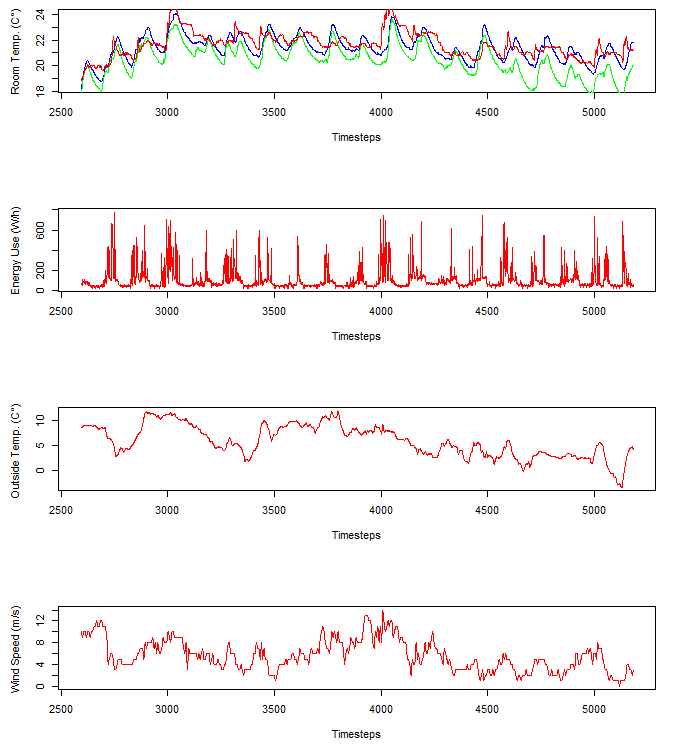
\includegraphics[scale=0.6]{Figures/temp_dataset}
	\decoRule
	\caption[Temperature Dataset]{Appliances Energy Prediction Dataset \parencite{Own or UCI???}}
	\label{fig:temp_dataset}
\end{figure}

\subsubsection{Sampling}
The data set contains datapoints measured between November and May. During this time period, it is observed, that the base temperature steadily rises. This poses the problem, that if the model is trained on data from November to March, with April as validation and May as test period, it is biased on the prevailing colder temperatures. To overcome this problem a special sampling technique was applied. In total six samples of the data set were created. A sample was created by randomly drawing one data point per hour over all datapoints. Four of these sample are then used for training, one for validation and one for testing. Using this sampling technique, the model is no longer biased on certain weather conditions but with the drawback, that the test set is not independent of the test and validation set.   

\subsubsection{Anomalies}
Again, the anomalies were embedded manually into the dataset. The anomalies are of type level shift, deviant cycles, variaton change and distribution-based aggregate anomaly. The anomalies were embedded into the room temperature variables (T1, T2, and T3) and the energy use variable. Figure \ref{fig:temp_anomalies} shows examples of the mentioned anomalies.

\begin{figure}[h]
	\centering
	\includegraphics[scale=0.7]{Figures/temp_anomalies}
	\decoRule
	\caption[Temperature Dataset Anomalies]{Examples of Embedded Anomalies \parencite{Own}}
	\label{fig:temp_anomalies}
\end{figure}

Since the test dataset only consists of around 3000 data points. It was used 3 times so that it does not have an unusual high density of anomalies. In the first instance, anomalies that only affected one variable were embedded. In the second instance, anomalies, that affected all 3 temperature variables, such as a deviant cycle, were embedded. On top, in the energy use variable, variation change anomalies were embedded.  In the third instance, distribution based anomalies, which affected T1 and T2, were embedded.

\subsection{Neural Networks}
Since the RNN did not show sufficient results in Experiment 1 when given a classification task, it was excluded from Experiment 2. The CNN, however, which had probably learned the patterns of the anomalies, was tested again. Since the anomalies in the training and test set are not as similar anymore as in Experiment 1, it is expected that the CNN classifier performs very poorly. 

\begin{table}[h]
	\caption{Configuration of Unupervised Learning in Exp. 2}
	\begin{center}
		\begin{tabular}{ | c | c | c | c |}
			\hline
			\thead{} & \thead{Input} & \thead{NN-Architecture} & \thead{Output} \\
			\hline
			\thead{CNN} &  288 past datapoints  & \makecell{3 1D-Convolutional Layers \\ 1 Max-Pooling Layers }  & \makecell{ 4 Dense Layers with \\ 1 regression outputs}   \\
			\hline
			\thead{RNN} &  288 past datapoints  & \makecell{3 LSTM Layers}  & \makecell{ 1 Dense Layers with \\ 4 regression outputs}  \\
			\hline
		\end{tabular}
		\label{Tab:Unupervised Learning2}
	\end{center}
\end{table}

Because of the complexity of the dataset, in the second experiment it was decided to use LSTM units instead of GRU in the RNN architecture. LSTM units generally provide more accurate results but use more memory and therefore more computation time \parencite{Lendave2021}. The designed neural network architecture consisted of 3 sequential layers of LSTM layers and one dense layer with four neurons. 
%https://analyticsindiamag.com/lstm-vs-gru-in-recurrent-neural-network-a-comparative-study/  

The CNN was designed as follows, three layers of one-dimensional convolutional layers were used. After the first layer, a max-pooling layer was added, to reduce the feature space and improve computation time. Since the CNN is expected to predict a time series, the feature space was not further reduced through max-pooling layers, since it would negatively affect the accuracy.  

\subsubsection{Learning}
The generator function for this experiment was configured as follows:

\begin{itemize}
	\item Lookback - 288 past data points: 12 days in the past
	\item Step - 1: no further subsampling is done
	\item Delay - 1: the next time step in the future is predicted
	\item Batch Size - 128 samples per batch
\end{itemize}

First experiments were done only using data from T1, T2, T3, energy use and outside temperature to predict T1 to T3 and appliances energy use. However, the achieved results were not satisfactory. The results were not accurate enough to predict the anomalies. It was theorized, that the training data did not contain enough information to reliably predict the future, therefore additional variables were added. Adding more variables to predict the future resulted in a better MAE. Finally, the following variables were used to make predictions: T1 to T5, energy use of appliances and ligths, outside temperature, air pressure and windspeed. As the anomlies, however, were only embedded into 4 out of the 10 variables, only the affected 4 were predicted.


\subsection{Results of Experiment 2}
Because the dataset was much more challenging, the reported scores are clearly inferior to Experiment 1. In total there were 13 anomalies to be detected in the test sets. The difference in F1-Score between the CNN and the RNN results from one anomaly which was not recognized by the CNN. However, training the RNN takes over 30 times longer than the CNN.

\begin{table}[h]
	\caption{Results of Experiment 2}
	\begin{center}
		\begin{tabular}{ | c | c | c | c |}
			\hline
			\thead{} & \thead{F1-Score} & \thead{Training Time} & \thead{Inference Time} \\
			\hline
			\thead{CNN Unsupervised} & 0.666666 & 172s   & 24s*   \\
			\hline
			\thead{RNN Unsupervised} & 0.727272 & 5420s   & 93s*   \\
			\hline
		\end{tabular}
		\label{Tab:Results2}
	\end{center}
\end{table}
* the inference time reported is on just one instance of the test dataset

The above reported results show the overall performance. Since the dataset was more complex than in the first experiment, the results are investigated further to show how the different architecture performed on the various anomalies and how accurate the predictions were on the different variables. First of all, the average error of the predicted variables are investigated further. The below results are reported from the first test set.

\begin{table}[h]
	\caption{MAE of Predictions}
	\begin{center}
		\begin{tabular}{ | c | c | c | c |}
			\hline
			\thead{} & \thead{CNN} & \thead{RNN} \\
			\hline
			\thead{T1} & 0.2712066° C   & 0.1741582° C    \\
			\hline
			\thead{T2} & 0.5236905° C    & 0.9009765° C    \\
			\hline
			\thead{T3} & 0.3210329° C    & 0.7244096° C    \\
			\hline
			\thead{Appliances} & 29.64146 Wh   & 72.91079 Wh   \\
			\hline
		\end{tabular}
		\label{Tab:Average_error}
	\end{center}
\end{table}

From Table \ref{Tab:Average_error}, it can be seen that the CNN outperforms the RNN on all variables except T1. The RNN, however, performs exceptionally well on T1. 
Comparing these results to the performance of the RNN on the first test set shows that only the anomalies that were embedded in T1 are detected. A similar picture emerges in the second test set, since the anomalies affect all 3 variables, a deflection should be visible on all three reported anomaly scores. However, the anomalies detected by the RNN were only visible in the anomaly score reported off T1. While the CNN is not as accurate on any of the variables as the RNN is on T1, this is how the CNN was outperformed. Out off the six anomalies embedded in the second test set, the CNN only recognized one, while the RNN recognized three out of six. On the third test set, both architecture types were able to recognize all anomalies.

Further, as expected, both architecture types were not able to find the variation change anomalies embedded in the variable appliances. The anomaly was constructed as when too many times the exact same value is reported. This anomaly type is with the necessary domain knowledge relatively easy to find.

\section{Experiment 3}
In the third experiment, a dataset that was dedicated to anomaly detection tasks was used. The achieved results can therefore be verified on previously achieved results.

\subsection{Dataset} \label{GHL_Dataset}
%https://arxiv.org/pdf/1612.06676.pdf
The dataset was introduced by Filonov et al. \parencite{Filonov2016}. The data was created by modelling a gasoil plant heating loop The GHL (Gasoil Heating Loop) model has three reservoirs: a receiving tank (RT), a heating tank (HT), and a collection tank (CT). The technological challenge is to heat gasoil in RT to 60 degrees Celsius, resulting in a viscosity sufficient for transmission to CT. In the model, the heating is done in stages. A fraction of gasoil is heated to 60 degrees Celsius in HT and then pumped back into RT to relax for a while. This technique is done until the RT temperature reaches 60 degrees Celsius. After that, the RT is poured into the CT. Following that, RT is refilled from an infinite source.

The training dataset consists of 19 variables and around 1.5 million datapoints with no anomalies, the most important, according to Filonov et al. \parencite{Filonov2016} are shown in Figure \ref{fig:GHL_data}. The sensors for RT level, RT temperature, and HT temperature are the first three variables. The remaining two variables relate to control signals for turning on/off the gasoil supply and turning on/off the heater.

For testing the trained models, Filonov et al. \parencite*{Filonov2016} provide 48 test sets, which are further decribed in Section \ref{GHL_Anomalies}

\begin{figure}[h]
	\centering
	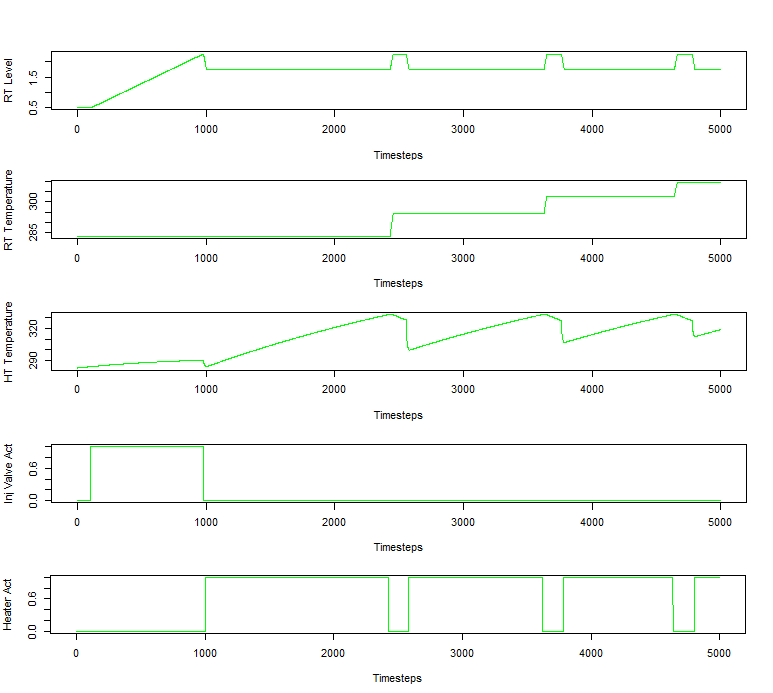
\includegraphics[scale=0.6]{Figures/GHL_data}
	\decoRule
	\caption[Most important var]{Examples of Embedded Anomalies \parencite{Own}}
	\label{fig:GHL_data}
\end{figure}

\subsubsection{Sampling}
The dataset intended for training contains 1.5 million data points, on top all 48 available test sets contain around 200'000 data points. The training of the neural networks and the evaluation of the test sets would therefore take a lot of time. Inspired by the work of Wen and Keyes \parencite*{Wen2019}, who took snapshots of length 50'000 and then downsampled them to a length of 1'024, the data should also be downsampled to save time. \textcolor{red}{ Downsampling  refers to reducing the number of data points in a time series. There are different techniques to achieve downsampling. The technique applied in this case is called decimation. Since the data contains many repeating data points, which have the same value, only every 10th datapoint was kept, which corresponds to a decimation by a factor of 10.} This greatly reduces the computation time, since the training dataset now contains only 150'000 data points while a test set contains 20'000 data points. On the downside, using this technique to downsample information is lost, which possibly effects the results of the chosen anomaly detection methods. Figure \ref{fig:downsample} shows how the variable RT Level behaves on 5'000 data points pre- and post-downsampling.

\begin{figure}[h]
	\centering
	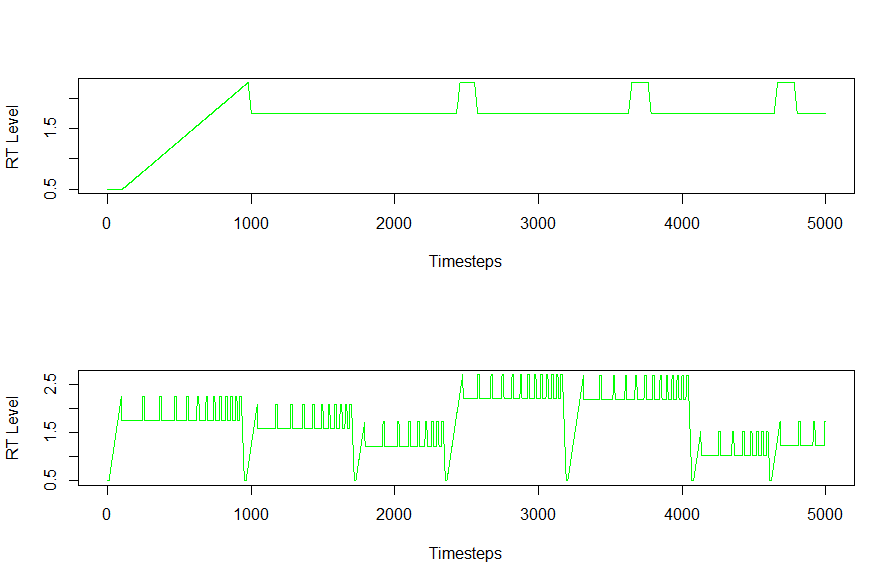
\includegraphics[scale=0.6]{Figures/downsample}
	\decoRule
	\caption[Effect of Downsampling]{Effect of Downsampling on RT Level \parencite{Own}}
	\label{fig:downsample}
\end{figure}

\newpage
\subsubsection{Anomalies} \label{GHL_Anomalies}
As anomalies cyber attacks were introduced. The anomalies each concern the variables RT Level and HT Temperature, which had been changed without authorisation. By setting the value for RT Level or HT Temperature to different levels and varying the the time of attack 48 test sets were created. Each test set contains only one anomaly of either type. Figure \ref{fig:anomaly_max_RT_level} and Figure \ref{fig:anomaly_max_HT_temp} give an example of the anomalies look like. In red, the variable Danger, which is the control variable that indicates the anomaly, is shown \footnote{In Figure \ref{fig:anomaly_max_HT_temp} the variable Danger was artificially lifted to a base level of 300 instead of 0 and multiplied by 10 for better visibility}.

\begin{figure}[h]
	\centering
	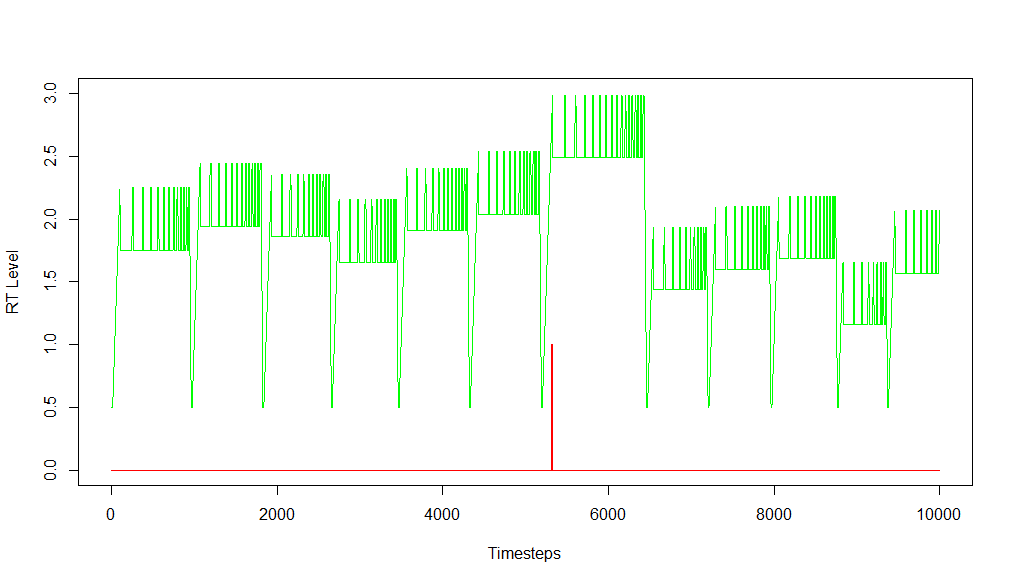
\includegraphics[scale=0.4]{Figures/anomaly_max_RT_level}
	\decoRule
	\caption[Attack on max-RT-level set point]{Attack on max-RT-level set point \parencite{Own}}
	\label{fig:anomaly_max_RT_level}
\end{figure}

\begin{figure}[h]
	\centering
	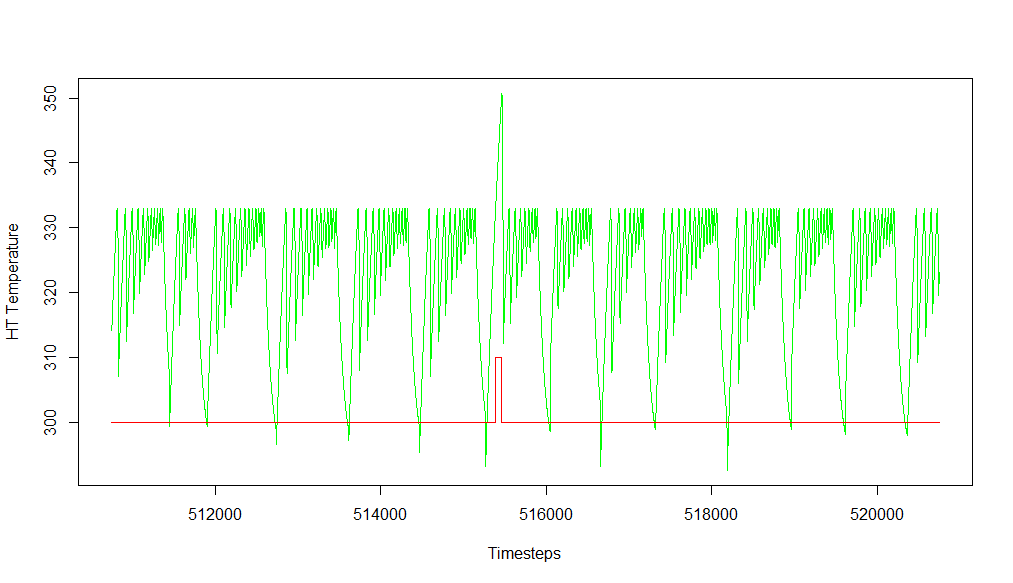
\includegraphics[scale=0.4]{Figures/anomaly_max_HT_temp}
	\decoRule
	\caption[Unauthorized change of max HT temperature]{Unauthorized change of max HT temperature \parencite{Own}}
	\label{fig:anomaly_max_HT_temp}
\end{figure}

Since the anomalies affect only the two above shown variables, the task for the neural networks was defined to predict the two above mentioned variables. Out of the past information of all 19 variables a neural network is expected to reliably predict the two monitored variables.

\subsection{Neural Networks}
\textcolor{red}{As described in Section \ref{GHL_Dataset}, the provided training dataset does not contain any anomalies, therefore only unsupervised training approaches are used. Wen and Keyes \parencite*{Wen2019} used the GHL dataset, for a supervised approach, but used part of the test set for training, therefore making it not possible to compare the results to works of Filonov et al. \parencite*{Filonov2016}.}

In Experiment 3, the chosen neural network architecture is again a LSTM. Since, Filonov et al. \parencite*{Filonov2016} use a LSTM network in their experiment, in order to be able to compare the experiments the same neural network architecture was chosen. However, Filonov et al. only report in their work, that two LSTM layers and a dropout layer were used. The exact configuration of the LSTM layers is not evident. Therefore, the number of units per layers was experimentally determined. \textcolor{red}{ Finally, 32 units and 24 units were used in the first and in the second layer respectively.} The dropout layer, which was added to reduce overfitting, was configured with a dropout rate of 0.1, which was adapted for this experiment. 

\begin{table}[h]
	\caption{Configuration of Unupervised Learning in Exp. 3}
	\begin{center}
		\begin{tabular}{ | c | c | c | c |}
			\hline
			\thead{} & \thead{Input} & \thead{NN-Architecture} & \thead{Output} \\
			\hline
			\thead{CNN} &  100 past datapoints  & \makecell{3 1D-Convolutional Layers \\ 2 Dropout Layers }  & \makecell{ 2 Dense Layers with \\ 1 regression outputs}   \\
			\hline
			\thead{RNN} &  100 past datapoints  & \makecell{2 LSTM Layers \\ 1 Dropout Layer}  & \makecell{ 1 Dense Layers with \\ 2 regression outputs}  \\
			\hline
		\end{tabular}
		\label{Tab:Unupervised Learning3}
	\end{center}
\end{table}

Some early experiments with a two-layered CNN yielded in poor results. Therefore, an additional convolutional layer was added. As in Experiment 2, initially included max-pooling layers were found to negatively impact the ability to accurately predict the required time series, therefore it was dispensed with completely. Since the CNN now also had a tendency to overfit, two dropout layers were added. 


\subsubsection{Learning}
The main challange when training the neural network was to determine an appropriate lookback. Initial experiments were carried out with 1000 - 5000 past data points that were considered. Although, the computation time increased significantly, the reported results were not satisfactory. Looking at the work of Wen and Keyes \parencite*{Wen2019}, who trained their network on snapshots of length 300 and applied a similarly rigorous sampling technique, the lookback paramter was set accordingly. Experiments with a lookback of between 300 and 500 past data points, improved not only the reported MAE, but also had a positive effect on computation time. While the results for the lookbacks between 300 and 500 were not significantly different, it was determined to use 300 because it resulted in the shortest computation time.
The generator function for this experiment was, therefore, configured as follows:

\begin{itemize}
	\item Lookback - 300 past data points: 1000 seconds in the past
	\item Step - 1: no further subsampling is done
	\item Delay - 1: the next time step in the future is predicted
	\item Batch Size - 128 samples per batch
\end{itemize}

\subsection{Results of Experiment 3}
As in the previously described experiments, the anomaly score was calculated as the difference between predicted value and actual value. Figure \ref{fig:rollmean} shows that calculating the different results in a graph with many peaks where the anomaly is not clearly visible. Filonov et al. \parencite*{Filonov2016} experienced the same problem and applied a exponential rolling mean on the calculated difference to smooth the outliers. The same technique is used, to smooth the difference calculated in Experiment 3, although only a simple rolling mean is calculated. \textcolor{red}{The lower graph of Figure \ref{fig:rollmean} shows the time series after the rolling mean was applied together with the Danger control variable in red and the applied threshold in blue.}

\begin{figure}[h]
	\centering
	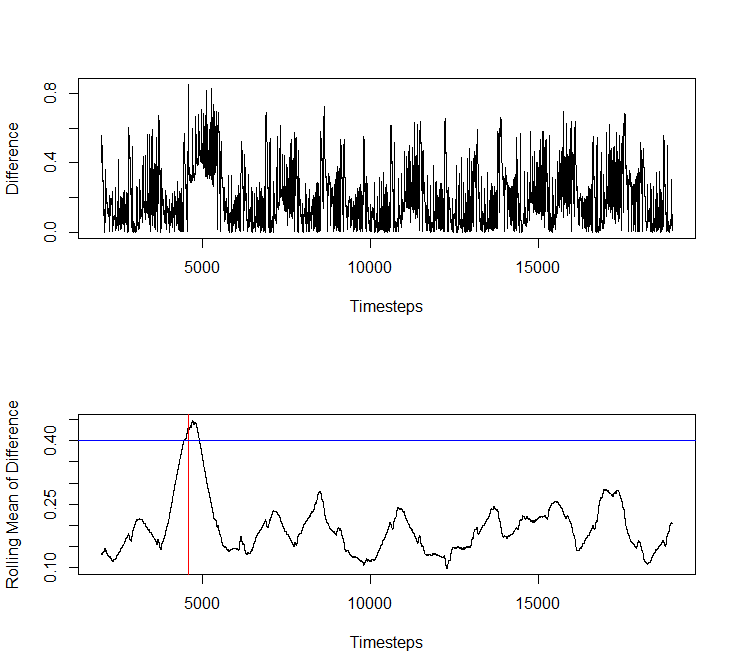
\includegraphics[scale=0.7]{Figures/Rollmean}
	\decoRule
	\caption[Effect of Rolling Mean Calculation]{Effect of Rolling Mean Calculation \parencite{Own}}
	\label{fig:rollmean}
\end{figure}

\newpage

% false positives at the start are not counted, they possibly exist due to a ramp up phase
\textcolor{red}{
Notable, when looking at the predictions on the test sets, is that every set had a ramp up beahviour where the predicted and actual did not match causing an anomaly at the start of all test sets. This behaviour was observed with both, the CNN and the RNN model, leading to the conclusion that this behaviour was created when the test set was generated. It was assumed, that this behaviour does not occur during operation. The anomalies caused by the ramp up phase were therefore not counted when calculating the final result. 
Further, when calculating the result, a series of anomalies that occur in quick succession are counted as just one anomaly as this refers to one of the identified flaws of the existing benchmarks (see Section \ref{Problems of Existing Benchmarks}). However, because of the down-sampling of the data and the application of a rolling mean to the predicted result, it would also no longer be possible to recognize the separate peaks caused by a series of anomalies. Since it is unknown whether Filonov et. al \parencite*{Filonov2016} used the same approach, it is possible that  better F1-Scores are achieved this way, but actually the task was simplified.\\
Although Wen and Keyes \parencite*{Wen2019} also used the GHL data for their experiment, the results cannot be compared as they used parts of the test set to train their model, meaning they could not evaluate their model on the whole test set.}
 \\

\begin{table}[h]
	\caption{Results of Experiment 3}
	\begin{center}
		\begin{tabular}{ | c | c | c | c |}
			\hline
			\thead{} & \thead{F1-Score} & \thead{Training Time} & \thead{Inference Time} \\
			\hline
			\thead{CNN Unsupervised } & 0.8696 & 142s   & 185s*   \\
			\hline
			\thead{RNN Unsupervised} & 0.9053 & 467s   & 530s*   \\
			\hline
			\thead{RNN Unsupervised**} & 0.872 & -   & -   \\
			\hline
		\end{tabular}
		\label{Tab:Results3}
	\end{center}
\end{table}

* the inference time reported is on just one instance of the test dataset\\
** Benchmark achieved by \Parencite{Filonov2016}



% Discuss labelling of Anomalies somewhere in respect to mislabelled ground truth. 

% Discuss influence of threshold on delay of recognition of anomaly

% Discuss importance of recognizing anomaly as fast as possible



